
\section{Problemformulering}
At designe og fremstille et éndimensionelt vognmonteret omvendt pendul, der ved hjælp af klassisk regulering og analog signalbehandling, skal kunne fastholde en forudbestemt vinkel af pendulet, samt at kunne kompensere for udefrakommende påvirkninger. 

\subsection{Formål}
Formålet med projektet er, at forene de opnåede fagligheder fra undervisningen på 3. semester. 
Alle fag fra undervisningen indgår i projektet, henholdsvis elektronik, elektromagnetisme, regulering, kredsløbsteknik og matematik.
Der tilstræbes at eftervise teorier fra semesterets fagligheder, der er anvendelige for at løse problemstillingerne i projektet. 


\subsection{Krav til rapporten stillet i projektoplæg}
Semestertema\footnote{Kilde: Semesterprojekt oplæg for 3. semester EE/ED 2016}: Måling og generering af elektromagnetiske felter kombineret med analog signalbehandling.
\begin{itemize}
\item Der skal udføres et projekt i overensstemmelse med semestertemaet.
\item Projektet skal indeholde fagligheder fra alle teorifagene. Fra elektrofysikken skal
magnetiske felter behandles.
\item Der skal foretages en grundig problemanalyse, der munder ud i en klar og entydig
problemformulering.
\item Produktet skal i videst mulig omfang baseres på lagerførte varer.
\end{itemize}

\subsection{Selvvalgte krav til projektet} \label{afs:kravspecifikation}
Udover de på forhånd stillede projektkrav, er der blevet foretaget yderligere selvvalgte krav, som fremgår herunder.
\begin{itemize}
\item Pendulet skal altid starte i ligevægtsposition, og må kun påvirkes små udefrakommende forstyrrelser.
\item Systemet skal kunne drives af to $7,4\si{\volt}$ LiPo batterier.
\item Sensoren til bestemmelse af pendulets vinkel skal anvende magnetfelter.
\item Systemet bygges på en eksisterende vogn med DC-motor, designet af en tidligere projekt gruppe. 
\item Systemet skal udelukkende være analogt. 
\end{itemize}

\subsection{Problemstilling}
Følgende problemstillinger ønskes besvaret:
\begin{itemize}
\item Hvilken fysisk model ligger til grund for et inverteret pendul?
\item Hvordan indgår vognens dynamik i den samlede regulering af systemet, og dimensioneringen deraf?
\item Hvordan måles pendulets vinkel ved hjælp af elektromagnetiske felter?
\item Hvordan beregnes en spoles magnetfelt og dets udbredelse?
\item Hvordan er den magnetiske kobling mellem 2 spoler?
\item Hvilken signalbehandling kræves for, at signalet fra transduceren kan anvendes til regulering? 
\item Hvordan forsynes kredsløbene korrekt ud fra den begrænsede batteriforsyning.    
\item Hvordan designes en motorstyring, der muliggør den ønskede kontrol af vognen?
\item Hvordan kan CAD og 3D-printer teknologi anvendes?
\item Hvordan opstilles systemets enkelte deles dynamik i en samlet reguleringsanalyse?
\item Hvordan dimensioneres regulatoren, således at systemet stabiliseres?
\end{itemize}

\subsection{Projektafgrænsning}
Følgende medtages ikke i rapporten og afgrænser projektarbejdet:
\begin{itemize}
\item Systemet er begrænset til kun at virke i én dimension.
\item Der ses bort fra den fysiske beskrivelse af elektromotoren.
\item Vogn samt tilhørende motor, hjul og gearing overtages fra tidligere projekt.
\item Der ses bort fra den termiske beregning af de valgte transistorer i motorstyringen.
\item Friktionskrafter på vogn, pendul m.m. er ikke medtaget i projektets omfang.   
\end{itemize}

\section{Løsningsmodel}
\begin{figure}[h!]
	\centering
	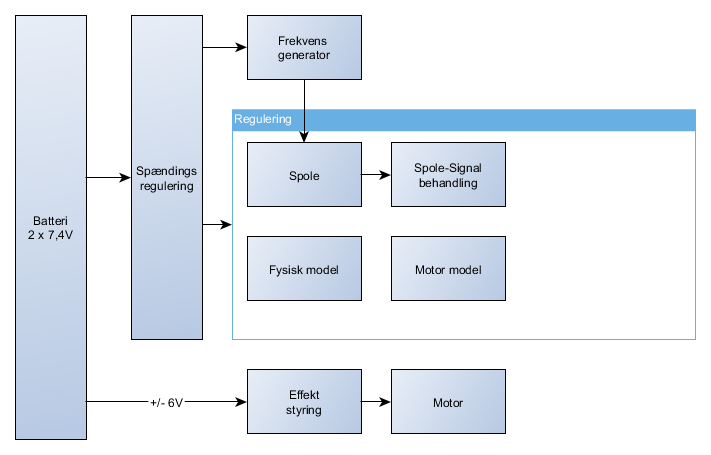
\includegraphics[width=.9\textwidth]{diagram/blokdiagram1.png}
	\caption{Systemets blokdiagram}
	\label{fig:blockdiagram1}
\end{figure}
\FloatBlock
I figur \ref{fig:blockdiagram1} ses blokdiagrammet over systemets opbygning. 
Da de selvvalgte krav gør rede for, at der ønskes batteridrift, startes der med to $7,4\volt$ batterier. 
Da de forskellige dele af systemet forsynes med forskellige spændinger, reguleres denne med en spændingsregulator og en shunt-regulator. Fra spændingsregulatoren fås der 14V, som sendes ind i signal-generatoren. 
Et firkant-signal som denne genererer (på $47\kilo\hertz$) bruges i afsenderspolen til, at inducere et signal i modtagerspolerne. 
Dette signal skal behandles, forstærkes og ensrettes, hvilket gøres i blokken 'Spole-Signalbehandling'.
Derefter sendes signalet ind i regulatoren, som er forsynet med $7\volt$ fra shunt-regulatoren. 
Motorstyringen modtager derefter det regulerede signal, og styrer strømmen, så motoren kan bevæge vognen for at holde pendulet oprejst. 
$9\volt$'s batteriet forsyner dele af motorstyringens, så den kan levere den ønskede strøm. 

\section{Læsevejledning}
Rapportens struktur er opdelt i hovedsektioner og undersektioner.
Opbygningen er taksonomisk både i kapitelstruktur og som helhed. 
Derudover afsluttes hvert kapitel med en opsummering og en delkonklusion.
For at få mest ud af rapporten, anbefales det at læse kapitlerne i rækkefølge.
Kapitlernes rækkefølge giver en naturlig gennemgang af systemet, både teoretisk og praktisk, og er baseret på dets signalvej.

\section{Proces- og arbejdsmetode}
Under projektforløbet, har fastlagte deadlines i et Gantt-diagram dannet oversigt. 
Arbejdsopgavernes omfang kunne derved bestemmes og afgrænses, hvilket har givet et godt arbejdsflow.
Ugentlige opsummeringsmøder og 'to-do'-lister har sørget for, at opgaverne blev lavet til tiden.

Det har også vist sig nødvendigt, at gøre brug af iterativ arbejdsmetode, idet den fulde kendskab af at kunne løse hvert problem ikke på forhånd kendes.

Den kollektive arbejdsmetode er blevet anvendt, hvor hvert gruppemedlems ressourcer og viden anvendes.
I forbindelse med den arbejdsproces, er en metode med fastlagte roller til dels blevet brugt.
Gruppen har ud fra deres viden, fastlagt sig i bestemte roller og herunder bestemte emner i rapporten.

Der er hele tiden taget højde for formidlingen af viden i rapporten, hvor målgruppen er studerende på 3. semester indenfor projektgruppens eget studieområde.
